\section{Opacità}\label{sec:opacità}
L'opacità è una misura della resistenza della materia al flusso radiativo, ovvero alla transizione della radiazione. È una sorta di sezione d'urto per unità di massa.
\[
\kappa = \kappa(\rho, T) \qquad [\kappa] = \si{cm^2.g^{-1}}
\]
L'equazione dell'opacità in un modello stellare si può riassumere nel seguente set di equazioni, che saranno sviscerate nei paragrafi seguenti:
\begin{equation}\label{eq:opacità}
    \kappa = \kappa(\rho, T) 
    \begin{cases} 
    \kappa_{BF} \propto 10^{25} Z(1 + X) \dfrac{\rho}{T^{3.5}} \\ 
    \kappa_{FF} \propto 10^{22} (X+Y)(1+X) \dfrac{\rho}{T^{3.5}} \\ 
    \kappa_{E} \propto 0.2 (1+X) \\ 
    \end{cases}
\end{equation}
I fenomeni che possono interferire con il passaggio di radiazione in una stella sono essenzialmente dovuti alla capacità degli elettroni di assorbire e/o deviare i fotoni, e si possono riassumere nei seguenti processi:
\begin{itemize}
    \item Assorbimento bound-bound (BB)
    \item Assorbimento bound-free(BF)
    \item Assorbimento free-free (FF)
    \item Scattering elettronico (E)
\end{itemize}
i quali sono spiegati di seguito. La rilevanza di questi processi dipende principalmente da tre fattori:
\begin{itemize}
    \item La composizione chimica del gas ($X$, $Y$, $Z$).
    \item La temperatura.
    \item La densità.
\end{itemize}
In particolare, è la temperatura a stabilire il livello di ionizzazione e dell'eccitazione di ogni specie chimica. In figura~\ref{fig:assorbimenti-stella} sono riportati i diversi processi di assorbimento in funzione della distanza dal centro stellare. È difficile una modellizzazione di tali processi, pertanto si utilizzano delle relazioni approssimate, note con il nome di \emph{leggi di Kramer}, che saranno mostrate nei seguenti paragrafi.

\begin{figure}
\centering
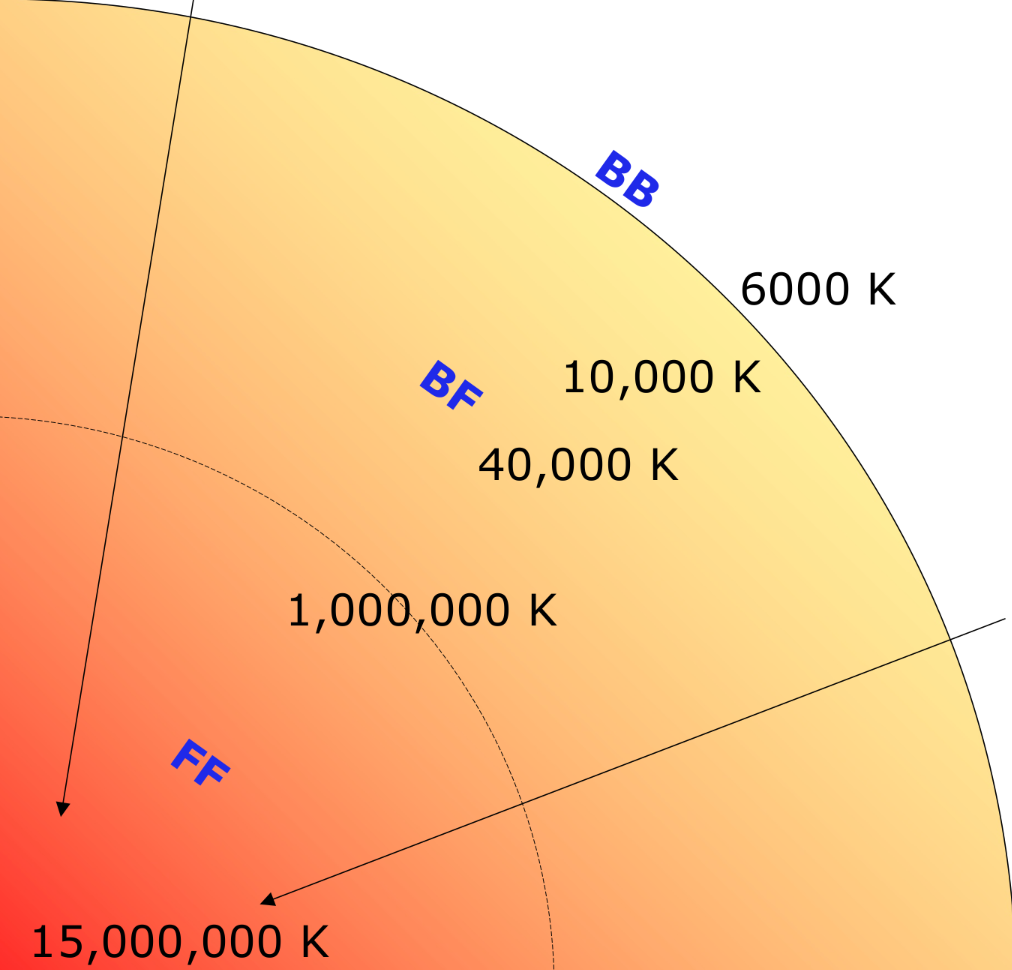
\includegraphics[width=0.3\textwidth]{immagini/assorbimenti-stella.png}
\caption{Processi di assorbimento preponderanti in funzione della distanza dal centro. Andando verso il centro della struttura le temperature aumentano, quindi il numero di atomi completamente ionizzati e il numero di elettroni liberi aumenta. In superficie domina il BB perché le temperature sono minori e gli atomi sono ancora non ionizzati. Andando verso il centro inizia a dominare il BF perché alcuni atomi sono parzialmente ionizzati. Verso l'interno domina il FF perché quasi tutti gli atomi sono ionizzati.}
\label{fig:assorbimenti-stella}
\end{figure}

\subsection{Assorbimento bound-bound (BB)}\label{sec:bound-bound}
Un elettrone legato a un atomo, in uno stato di energia $E_1$, cattura un fotone e passa a uno stato eccitato $E_2$ \emph{rimanendo legato all'atomo}. Il fotone catturato ha energia:
\begin{equation}
    h \nu_{BB} = E_2 - E_1
\end{equation}
questo effetto \emph{non} è rilevante negli interni stellari, siccome quasi tutti gli atomi sono completamente ionizzati a causa delle elevate temperatura (fig.~\ref{fig:assorbimenti-stella}). Tuttavia, questo fenomeno è cruciale nell'\emph{atmosfera} stellare ed è responsabile della formazione delle righe di assorbimento spettrale.

In particolare, tale fenomeno avviene a una determinata lunghezza d'onda, ovvero:
\begin{equation}\label{eq:lunghezza-BB}
    \lambda_{12} = h \dfrac{c}{E_2 - E_1}
\end{equation}

Come detto, essendo questo fenomeno non rilevante negli interni stellari, non viene considerato nell'equazione dell'opacità.

\subsection{Assorbimento bound-free (BF)}\label{sec:bound-free}
Un elettrone legato a energia $E_1$ cattura un fotone e diventa libero, con energia $E_\infty$, producendo uno ione. Il fotone catturato ha energia
\begin{equation}
    h \nu_{BF} = E_\infty - E_1 > \chi_\textup{ion}
\end{equation}
dove $\chi_\textup{ion}$ è l'energia di ionizzazione dell'atomo. 

Tale fenomeno, dunque, avviene a una \emph{lunghezza d'onda} minore di una determinata soglia (di conseguenza, per la \emph{frequenza}, ho un limite inferiore ma non superiore), ovvero:
\begin{equation}\label{eq:lunghezza-BF}
    \lambda < \lambda_\textup{soglia}
\end{equation}

Rispetto all'atmosfera, in cui domina il BB, andando verso il centro inizierà progressivamente a dominare il BF a causa dell'aumento della temperatura e del fatto che  alcuni atomi iniziano a essere parzialmente ionizzati (fig~\ref{fig:assorbimenti-stella}). La corrispondente legge di Kramer, che compare nella~\eqref{eq:opacità}, si può scrivere nella seguente maniera:
\begin{equation}
    \kappa_{BF} \propto 10^{25} Z (1+X) \dfrac{\rho}{T^{3.5}}
\end{equation}
L'opacità $\kappa_{BF}$ dipende da Z, ovvero dall'abbondanza degli elementi più pesanti dell'elio, perché affinché il BF possa avvenire è necessario che siano ancora presenti degli atomi con elettroni legati. A causa della ionizzazione dell'idrogeno e dell'elio verso gli interni stellari, si possono trovare elettroni legati solamente negli elementi più pesanti.

\subsection{Assorbimento free-free (FF)}\label{sec:free-free}
Un elettrone libero, di energia $E_1$, cattura un fotone e la sua energia aumenta a $E_2$. Il fotone catturato ha energia:
\begin{equation}
    h \nu_{FF} = E_2 - E_1
\end{equation}
senza restrizioni come nei casi precedenti, perché il sistema non è legato. Questo processo è dominante negli interni stellari, perché lì la temperatura è così elevata che gli atomi sono tutti ionizzati (fig~\ref{fig:assorbimenti-stella}). Non ci sono limitazioni alla lunghezza d'onda in cui tale fenomeno può avvenire. La corrispondente legge di Kramer, che compare nella~\eqref{eq:opacità}, si può scrivere nella seguente maniera:
\begin{equation}
   \kappa_{FF} \propto 10^{22} (X+Y) (1+X) \dfrac{\rho}{T^{3.5}}
\end{equation}
L'opacità $\kappa_{FF}$ \emph{dipende da X e Y} perché il FF dipende dagli elettroni liberi e l'idrogeno e l'elio, che sono ionizzati alle alte temperature degli interni stellari, sono di gran lunga gli elementi più abbondandi, e dunque anche i principali fornitori di elettroni liberi.

\subsection{Scattering elettronico (E)}\label{sec:electron-scattering}
Un elettrone libero interagisce con un fotone, cambiando al propria traiettoria. Non si tratta di un reale assorbimento, ma agisce comunque come un effetto di opacità perché essendo il fotone deviato dal fascio, l'intensità del fascio stesso diminuisce. La corrispondente legge di Kramer, che compare nella~\eqref{eq:opacità}, si può scrivere nella seguente maniera:
\begin{equation}
    \kappa_E \propto 0.2(1+X)
\end{equation}
Si noti come \emph{non} ci sia dipendenza dalla temperatura $T$ e dalla densità $\rho$ e come esso \emph{dipende solo da X}, poiché l'idrogeno è l'elemento più abbondante. Lo scattering diventa dominante solamente ad alte temperature, perché per gli altri processi $\kappa \propto T^{-3.5}$.

\subsection{Recap}
Per riassumere l'andamento dell'opacità rappresentato dall'eq.~\eqref{eq:opacità}, facciamo riferimento alla figura~\ref{fig:opacità}. Possiamo notare che, in generale, l'opacità aumenta con la densità, infatti si ha $\kappa \propto \rho$. Inoltre si può notare che per temperature nelle regioni a $T \sim \SI{e4}{K}$ l'opacità aumenta, infatti questa è la finestra di temperatura che corrisponde alla \emph{ionizzazione dell'idrogeno}. Ovviamente, se l'idrogeno \emph{non} è ionizzato, allora i processi BF, FF ed E sono impossibili, poiché necessitano di elettroni liberi. D'altra parte, all'aumentare della temperatura, dunque al grado di ionizzazione degli elementi presenti nella struttura stellare, l'opacità decresce secondo~\eqref{eq:opacità}, con $\kappa \propto T^{-3.5}$. Ad altissime temperature, invece, domina lo scattering elettronico e la curva si appiattisce, come ci si  aspetta.

\begin{figure}
    \centering
    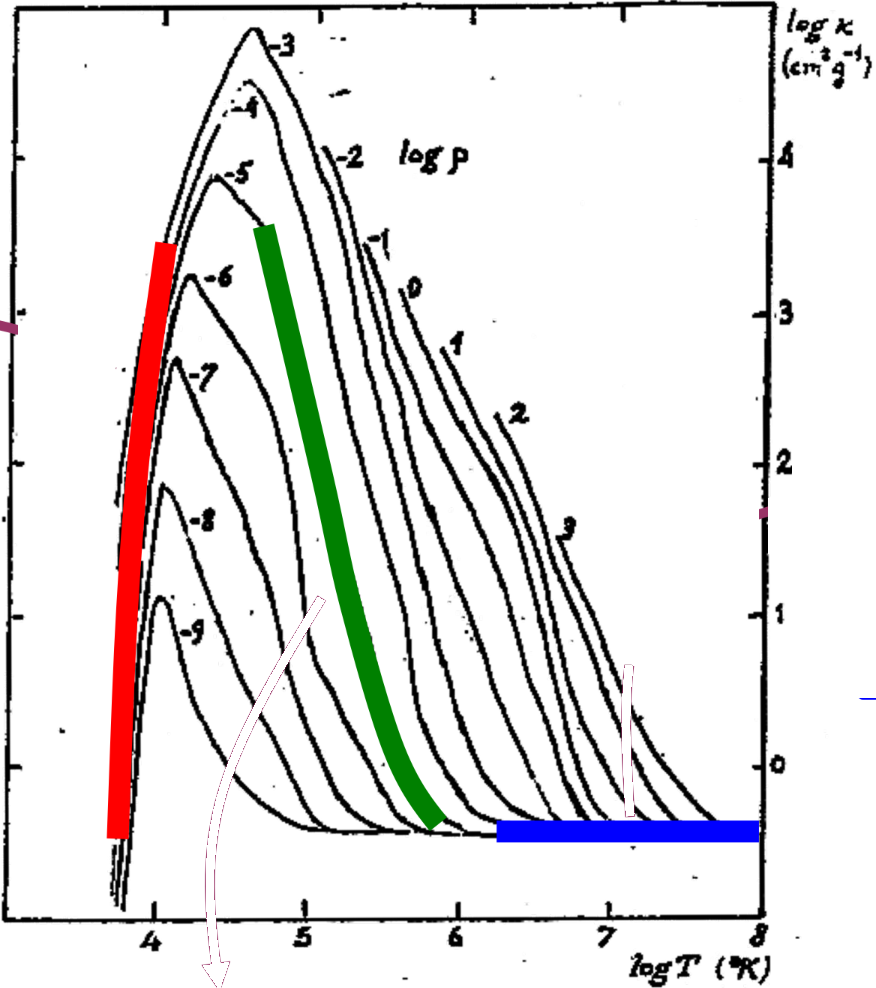
\includegraphics[width=0.35\textwidth]{immagini/opacita.png}
    \caption{Diagramma $\log \kappa$ -- $\log T$. Sono rappresentate curve a diverso $\log \rho$. A $T \sim \SI{e4}{K}$, curva rossa, l'opacità aumenta perché è in atto la ionizzazione dell'idrogeno. Nella curva verde si ha $\kappa \propto T^{-3.5}$ come indicato dalla eq.~\eqref{eq:opacità}. Nella curva blu domina lo scattering elettronico e l'opacità è costante come atteso.}
    \label{fig:opacità}
\end{figure}